\section{Experiments and Evaluation}
TODO: dataset
\subsection{Dimension reduction}
Our first set of experiments featured the basic dimension reduction method, without the modifications for compression. We were looking to verify that the required reconstruction information was present within the lower dimensional representation created by the feature extractor. (TODO include bitrate) The qualitative results can be seen in Figure 1. \\
We also utilized our latent loss scheme by pre-training on image reconstruction before training on the latent loss. The results can be seen in Figure 2.
\begin{figure}[H]
    \centering
    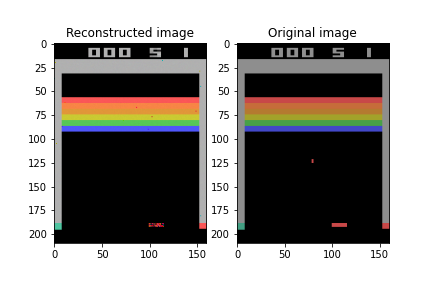
\includegraphics[width=0.6\textwidth]{images/orig_reconstructed0.0.png}
    \caption{Baseline method (no compression) with decoder trained on MSE for 10,000 iterations}
    \label{fig:baseline_MSE}
\end{figure}
\begin{figure}[H]
    \centering
    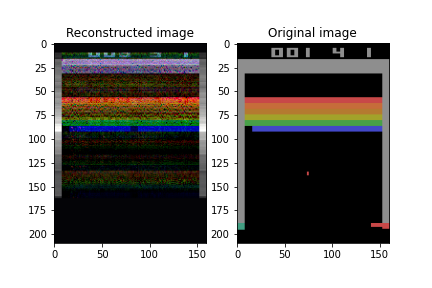
\includegraphics[width=0.6\textwidth]{images/orig_reconstructed_rl3.0.png}
    \caption{Baseline method (no compression) with decoder trained on MSE for 10,000 iterations, then latent MSE for 10,000 iterations}
    \label{fig:baseline_MSE_latent}
\end{figure}
